\subsection{Bayes Theorem}

Up until now we have used \Cref{fig:analysis:bayesian-network:abc} as an example Bayesian network. A more realistic network is illustrated in \Cref{fig:analysis:bayesian-network:sample} where $K = \{Fraud, Age, Sex, Gas, Jewelry\}$, $E = \{\{Fraud, Gas\}, \{Fraud, Jewelry\}, \{Age, Jewelry\}, \{Sex, Jewelry\}\}$ and P can be defined as in \Cref{tbl:analysis:bayesian-network:sample-tables-1,tbl:analysis:bayesian-network:sample-tables-2,tbl:analysis:bayesian-network:sample-tables-3}. The network models credit card fraud. From the network we can see, that if there is credit card fraud then there is a chance of gas or jewelry being bought. The chance of jewelry being bought is also affected by the age and the sex of the purchaser.

\begin{figure}[h!]
\centering
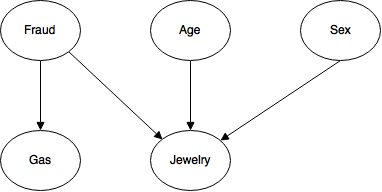
\includegraphics[width=0.5\textwidth]{images/sample_bayesian_network}
\caption{Sample Bayesian network. The network consist of five nodes, \ie~five variables. The Fraud node influence the Gas and Jewelry nodes and the Jewelry node is further influenced by the Sex and Age nodes~\cite{stephenson2000introduction}.}
\label{fig:analysis:bayesian-network:sample}
\end{figure}

\begin{table}[h!]
\centering
\caption{Probability tables for the Fraud, Gas and Sex nodes in the network illustrated in \Cref{fig:analysis:bayesian-network:sample}. Values are from~\cite{stephenson2000introduction}.}
\label{tbl:analysis:bayesian-network:sample-tables-1}
\begin{tabular}{ccc}
\begin{tabular}{c}
\textbf{Fraud}   \\
\begin{tabular}{cc}
Yes   & No \\ \hline
0.00001 & 0.99999
\end{tabular}
\end{tabular}
&
\begin{tabular}{c}
\textbf{Age}   \\
\begin{tabular}{ccc}
< 30 & 30-50 & > 50  \\ \hline
0.25 & 0.4 & 0.35
\end{tabular}
\end{tabular}
&
\begin{tabular}{c}
\textbf{Sex}   \\
\begin{tabular}{cc}
Male   & Female \\ \hline
0.5    & 0.5
\end{tabular}
\end{tabular}
\end{tabular}
\end{table}

\begin{table}[h!]
\centering
\caption{Conditional probability table for the Gas node in the network illustrated in \Cref{fig:analysis:bayesian-network:sample}. Values are from~\cite{stephenson2000introduction}.}
\label{tbl:analysis:bayesian-network:sample-tables-2}
\begin{tabular}{c}
\textbf{Gas}   \\
\begin{tabular}{l|cc}
             & Gas = Yes   & Gas = No \\ \hline
Fraud = Yes  & 0.2         & 0.8 \\
Fraud = No   & 0.01       & 0.99 \\
\end{tabular}
\end{tabular}
\end{table}

\begin{table}[h!]
\centering
\caption{Conditional probability table for the Jewelry node in the network illustrated in \Cref{fig:analysis:bayesian-network:sample}. Values are from~\cite{stephenson2000introduction}.}
\label{tbl:analysis:bayesian-network:sample-tables-3}
\begin{tabular}{c}
\textbf{Jewelry} \\
\begin{tabular}{l|c}
Age           & \begin{tabularx}{0.8\textwidth}{Y|Y|Y} < 30 & 30 - 50 & > 50 \end{tabularx} \\ \hline
Fraud         & \begin{tabularx}{0.8\textwidth}{YY|YY|YY} Yes & No & Yes & No & Yes & No \end{tabularx} \\ \hline
Sex           & \begin{tabularx}{0.8\textwidth}{YY|YY|YY|YY|YY|YY} M & F & M & F & M & F & M & F & M & F & M & F \end{tabularx} \\ \hline
Jewelry = Yes & \begin{tabularx}{0.8\textwidth}{YY|YY|YY|YY|YY|YY} $\frac{1}{20}$ & $\frac{1}{20}$ & $\frac{1}{10000}$ & $\frac{1}{2000}$ & $\frac{1}{20}$ & $\frac{1}{20}$ & $\frac{1}{2500}$ & $\frac{1}{500}$ & $\frac{1}{20}$ & $\frac{1}{20}$ & $\frac{1}{5000}$ & $\frac{1}{1000}$ \end{tabularx} \\
Jewelry = No  & \begin{tabularx}{0.8\textwidth}{YY|YY|YY|YY|YY|YY} $\frac{19}{20}$ & $\frac{19}{20}$ & $\frac{9999}{10000}$ & $\frac{1999}{2000}$ & $\frac{19}{20}$ & $\frac{19}{20}$ & $\frac{2499}{2500}$ & $\frac{499}{500}$ & $\frac{19}{20}$ & $\frac{19}{20}$ & $\frac{4999}{5000}$ & $\frac{999}{1000}$ \end{tabularx}
\end{tabular}
\end{tabular}
\end{table}

Given the network illustrated in \Cref{fig:analysis:bayesian-network:sample} we could be interested in computing $P(Fraud|Jewelry = Yes, Gas = No, Sex = Male, Age = < 30)$, that is, the probabilities of fraud happening when we have observed, that a male purchaser younger than 30 years have bought jewelry and have not bought gas.

We compute this using Bayes' theorem which is defined as:

\begin{equation}
P(A|B) = \frac{P(B|A)P(A)}{P(B)}
\end{equation}

More specifically, we want to compute the following. Note that for readability purposes the names of the variables and the states have been shortened to their initial letter.

\begin{equation*}
P(F=Y|J = Y, G = N, S = M, A = < 30)
\end{equation*}
\begin{equation*}
\begin{split}
&= \frac{P(J = Y, G = N, S = M, A = < 30|F=Y) \cdot P(F=Y)}{P(J = Y, G = N, S = M, A = < 30)} \\
&= \frac{P(J = Y, S = M, A = < 30|F=Y) \cdot P(G=N|F=Y) \cdot P(F=Y)}{P(J = Y, G = N, S = M, A = < 30)}
\end{split}
\end{equation*}

According to \Cref{eq:analysis:bayesian-network:prod} we can write this as

\begin{equation*}
P(F=Y|J = Y, G = N, S = M, A = < 30)
\end{equation*}
\begin{equation*}
= \frac{P(J = Y, S = M, A = < 30|F=Y) \cdot P(G=N|F=Y) \cdot P(F=Y)}{P(J=Y|F=Y,S=M,A=<30) \cdot P(G=N|F=Y) \cdot P(S=M) \cdot P(A=<30)}
\end{equation*}

Then we substitute with the probabilities from our probability tables and conditional probability tables.

\begin{equation*}
P(F=Y|J = Y, G = N, S = M, A = < 30)
\end{equation*}
\begin{equation*}
= \frac{\frac{1}{20} \cdot 0.8 \cdot 0.00001}{\frac{1}{20} \cdot 0.8 \cdot 0.5 \cdot 0.25} =
\end{equation*}
%%% Local Variables:
%%% mode: latex
%%% TeX-master: "../../master"
%%% End:
